\subsection{The Impact of RNA-Binding on IFIT2-pIB Interaction} \label{subsec:The Impact of RNA-Binding on IFIT2-pIB Interaction}
\subsubsection{The Generation of Bovine IFIT2 RNA-Binding Mutant} \label{The Generation of Bovine IFIT2 RNA-Binding Mutant}
Using published data about hIFIT2 rna-binding mutant

Difficulty of using alpha-fold with IFIT2 due to the swap domain

Using SWISS-MODEL to predict bIFIT2 structure from published hIFIT2 structures

Alignment of both structures, assessment of electrostatic charges and establishment of residues to be mutated

Primer design and mutagenesis procedure based on published hIFIT2 RNA-binding mutant paper

\begin{figure}
    \centering
    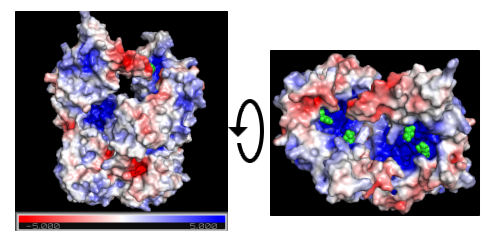
\includegraphics[width=1\linewidth]{09. Chapter 4/Figs/04. IFIT2-RNA binding mutant/01. structure.png}
    \caption[ifit2 mutant structure]{\textbf{bifit2 mutant structure.} redo this figure}
    \label{fig:ifit2 mutant structure}
\end{figure}

\subsubsection{Bovine IFIT2 RNA-Binding Mutant and RSV pIBs} \label{Bovine IFIT2 RNA-Binding Mutant and RSV pIBs}

\begin{figure}
    \begin{subfigure}{0.495\textwidth}
        \caption{}
        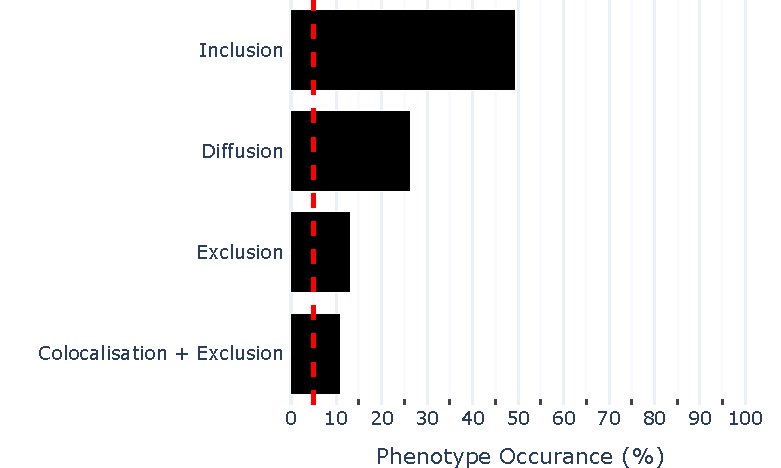
\includegraphics[width=1\linewidth]{09. Chapter 4/Figs/04. IFIT2-RNA binding mutant/02. pIB/01. bar_bi2f24_hnhp.pdf} 
    \end{subfigure}
    \begin{subfigure}{0.495\textwidth}
        \caption{}
        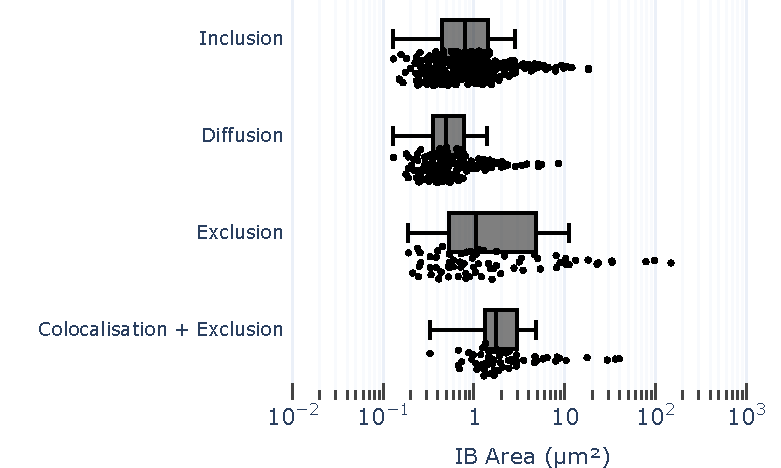
\includegraphics[width=1\linewidth]{09. Chapter 4/Figs/04. IFIT2-RNA binding mutant/02. pIB/02. box_bi2f24_hnhp.pdf}
    \end{subfigure}
    \caption[Diverse Phenotypic Interactions of Bovine IFIT2 RNA-Binding Mutant with Human RSV Pseudo Inclusion Bodies (pIBs) in the VERO Cell Line.]{\textbf{Diverse Phenotypic Interactions of Bovine IFIT2 RNA-Binding Mutant with Human RSV Pseudo Inclusion Bodies (pIBs) in the VERO Cell Line.} Vero cells were transfected with hRSV N and P, along with bovine IFIT2-FLAG RNA-binding mutant containing plasmids using TransIT-X2 and were fixed after 24 hours. Cells were labeled with anti-RSV N and anti-FLAG antibodies and imaged on confocal microscope. Panel (a) shows percentual proportions of observed phenotypes between hRSV pseudo inclusion bodies and exogenous bovine IFIT2-FLAG RNA-binding mutant (548 observations), with the red dotted line denoting the 5\% threshold, marking phenotypes considered relevant above this limit. Panel (b) shows the IB area in \(\mu m^2\) per observed relevant phenotype.}
    \label{fig:Diverse Phenotypic Interactions of Bovine IFIT2 RNA-Binding Mutant with Human RSV Pseudo Inclusion Bodies (pIBs) in the VERO Cell Line}
\end{figure}

\begin{figure}
    \centering
    \includegraphics[width=1\linewidth]{09. Chapter 4/Figs/04. IFIT2-RNA binding mutant/02. pIB/03. bi2f24-hnhp.pdf}
    \caption[Representative Images of Diverse Phenotypic Interactions of Bovine IFIT2 RNA-Binding Mutant with Human RSV Pseudo Inclusion Bodies (pIBs) in the VERO Cell Line.]{\textbf{Representative Images of Diverse Phenotypic Interactions of Bovine IFIT2 RNA-Binding Mutant with Human RSV Pseudo Inclusion Bodies (pIBs) in the VERO Cell Line.}  Vero cells were transfected with bRSV N and P, along with bovine IFIT2-FLAG RNA-binding mutant containing plasmids using TransIT-X2 and were fixed after 24 hours. Cellular nuclei were stained with DAPI (yellow), and cells were double-labeled with anti-RSV N (cyan) and anti-FLAG (magenta) antibodies. This figure showcases representative examples of relevant phenotypes in the interaction between exogenous bovine IFIT2-FLAG RNA-binding mutant and hRSV pseudo inclusion bodies. These phenotypes are presented in descending order based on their percentage proportions. The scale bar indicates 2 \(\mu m\).}
    \label{fig:Representative Images of Diverse Phenotypic Interactions of Bovine IFIT2 RNA-Binding Mutant with Human RSV Pseudo Inclusion Bodies (pIBs) in the VERO Cell Line}
\end{figure}

49 27 13 11
0.8 0.5 1 1.8

\begin{figure}
    \begin{subfigure}{0.495\textwidth}
        \caption{}
        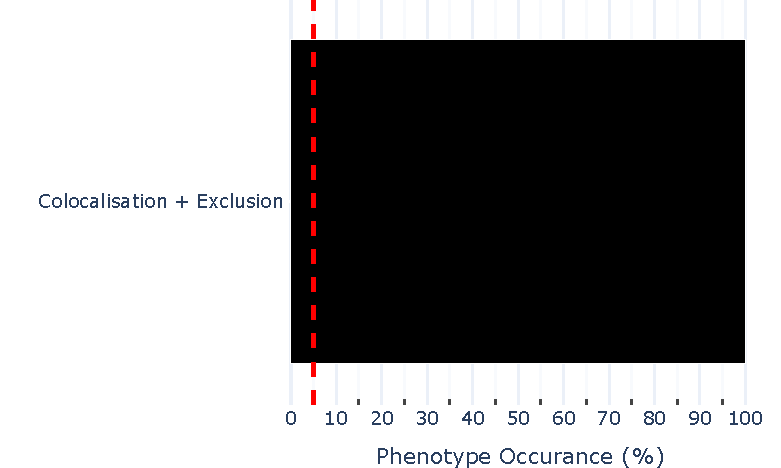
\includegraphics[width=1\linewidth]{09. Chapter 4/Figs/04. IFIT2-RNA binding mutant/02. pIB/04. bar_bi2f24_bnbp.pdf} 
    \end{subfigure}
    \begin{subfigure}{0.495\textwidth}
        \caption{}
        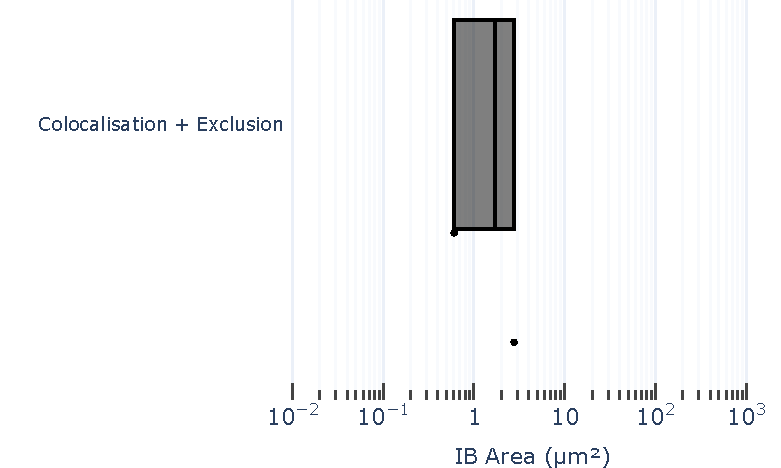
\includegraphics[width=1\linewidth]{09. Chapter 4/Figs/04. IFIT2-RNA binding mutant/02. pIB/05. box_bi2f24_bnbp.pdf}
    \end{subfigure}
    \caption[Diverse Phenotypic Interactions of Bovine IFIT2 RNA-Binding Mutant with Bovine RSV Pseudo Inclusion Bodies (pIBs) in the VERO Cell Line.]{\textbf{Diverse Phenotypic Interactions of Bovine IFIT2 RNA-Binding Mutant with Bovine RSV Pseudo Inclusion Bodies (pIBs) in the VERO Cell Line.} Vero cells were transfected with bRSV N and P, along with bovine IFIT2-FLAG RNA-binding mutant containing plasmids using TransIT-X2 and were fixed after 24 hours. Cells were labeled with anti-RSV N and anti-FLAG antibodies and imaged on confocal microscope. Panel (a) shows percentual proportions of observed phenotypes between bRSV pseudo inclusion bodies and exogenous bovine IFIT2-FLAG RNA-binding mutant (2 observations), with the red dotted line denoting the 5\% threshold, marking phenotypes considered relevant above this limit. Panel (b) shows the IB area in \(\mu m^2\) per observed relevant phenotype.}
    \label{fig:Diverse Phenotypic Interactions of Bovine IFIT2 RNA-Binding Mutant with Bovine RSV Pseudo Inclusion Bodies (pIBs) in the VERO Cell Line}
\end{figure}

\begin{figure}
    \centering
    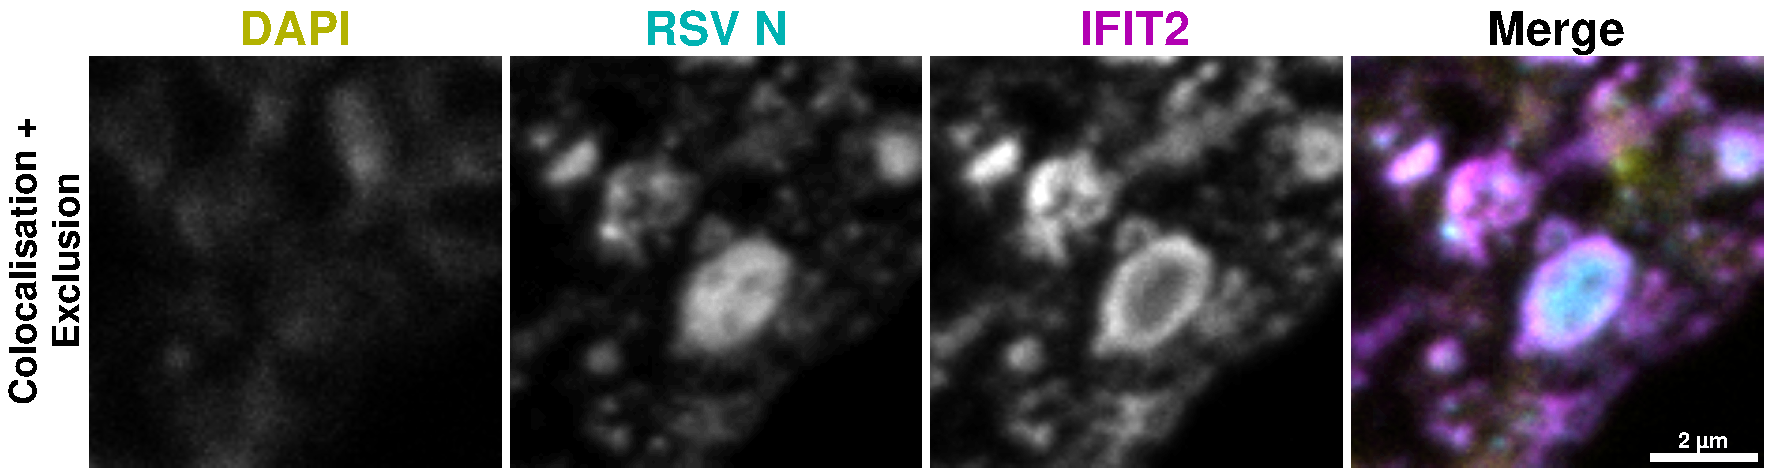
\includegraphics[width=1\linewidth]{09. Chapter 4/Figs/04. IFIT2-RNA binding mutant/02. pIB/06. bi2f24-bnbp.pdf}
    \caption[Representative Images of Diverse Phenotypic Interactions of Bovine IFIT2 RNA-Binding Mutant with Bovine RSV Pseudo Inclusion Bodies (pIBs) in the VERO Cell Line.]{\textbf{Representative Images of Diverse Phenotypic Interactions of Bovine IFIT2 RNA-Binding Mutant with Bovine RSV Pseudo Inclusion Bodies (pIBs) in the VERO Cell Line.}  Vero cells were transfected with bRSV N and P, along with bovine IFIT2-FLAG RNA-binding mutant containing plasmids using TransIT-X2 and were fixed after 24 hours. Cellular nuclei were stained with DAPI (yellow), and cells were double-labeled with anti-RSV N (cyan) and anti-FLAG (magenta) antibodies. This figure showcases representative examples of relevant phenotypes in the interaction between exogenous bovine IFIT2-FLAG RNA-binding mutant and bRSV pseudo inclusion bodies. These phenotypes are presented in descending order based on their percentage proportions. The scale bar indicates 2 \(\mu m\).}
    \label{fig:Representative Images of Diverse Phenotypic Interactions of Bovine IFIT2 RNA-Binding Mutant with Bovine RSV Pseudo Inclusion Bodies (pIBs) in the VERO Cell Line}
\end{figure}

100
1.8

\subsubsection{Summary}
We have described how bovine IFIT2 RNA-binding mutant was designed based on the published human IFIT2 RNA-binding mutant data (needs to be annotated more). Overexpression of bovine IFIT2 RNA-binding mutant yields cellular distribution and morphology similar to what was observed with overexpressing human IFIT2-FLAG, suggesting that the mutant proteins are not toxic to the cells. In the first experiment where we were looking at interaction between bovine IFIT2 RNA-binding mutant and human pseudo inclusion bodies we saw several phenotypes. We observed bovine IFIT2 RNA-binding mutant being excluded from small and big pIBs and pIB associated filamentous network, while fully or partially colocalising with other pIBs. In a subsequent experiment we observed only colocalization and inclusion formation. When assessing the interaction between bovine IFIT2 RNA-binding mutant and human pIBs formed using wild-type human RSV P and GFP-tagged human RSV N, we observed consistently in two experiments that bovine IFIT2 RNA-binding mutant colocalises to the pIB structures.